\section{\textcolor{unibablueI}{Location Info}}

\begin{center}
\begin{tikzpicture}[yscale=-0.1, xscale=0.1, node distance=1mm,inner sep = 0pt, outer sep = 0pt]
\tikzset{grid/.style={gray,very thin,opacity=1}}
\tikzstyle{default}=[anchor=north west]
\tikzstyle{copyright}=[fill=unibayellowV, inner sep=1pt, outer sep=1pt, anchor=south west, rounded corners, opacity=.8, font=\footnotesize]
\tikzstyle{location}=[anchor=north west, align=center, fill=unibablueV, opacity=0.8, rounded corners, inner sep=1pt]
\tikzstyle{room}=[anchor=north west, align=center, inner sep=1pt, font=\footnotesize]
    
%\draw[grid] (0,0) grid (10*\textwidth,10*\textheight);
\node[default](p1) at (0,0) {
          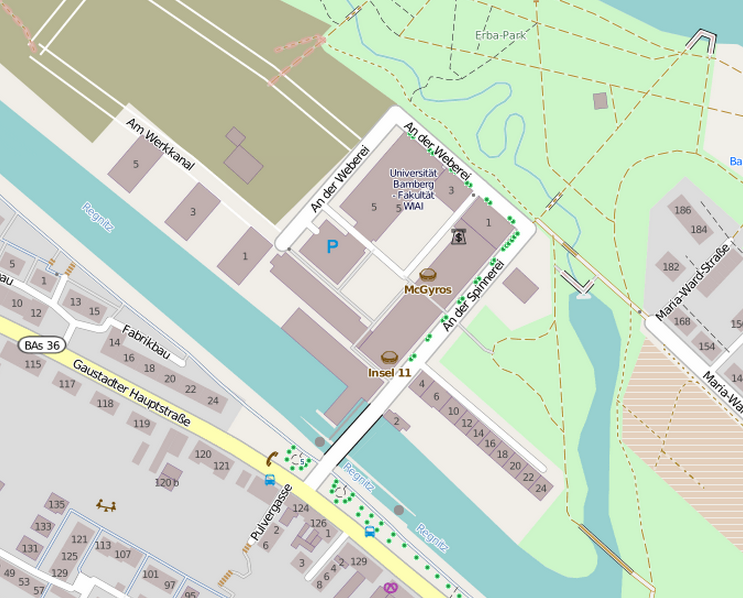
\includegraphics[width=\textwidth]{images/map2.png}
      
    };
\node[copyright](cr) at (p1.south west){\textcopyright~ {OpenStreetMap} contributors};    
   
%\draw[grid] (0,0) grid (10*\textwidth,6*\textheight);
\draw[ultra thick, unibaredI](46,21) circle (4cm);
\draw[ultra thick, unibablueII](41.5,59.5) circle (2cm);
\draw[ultra thick, unibablueII](30.3,53.6) circle (2cm); 
\node[location] at(33, 49){Bus stop\\ ``Spinnerei''}; 
\node[location] at(51, 19){University};  
   
   \node[default] (p2) [below=1cm of p1] {
         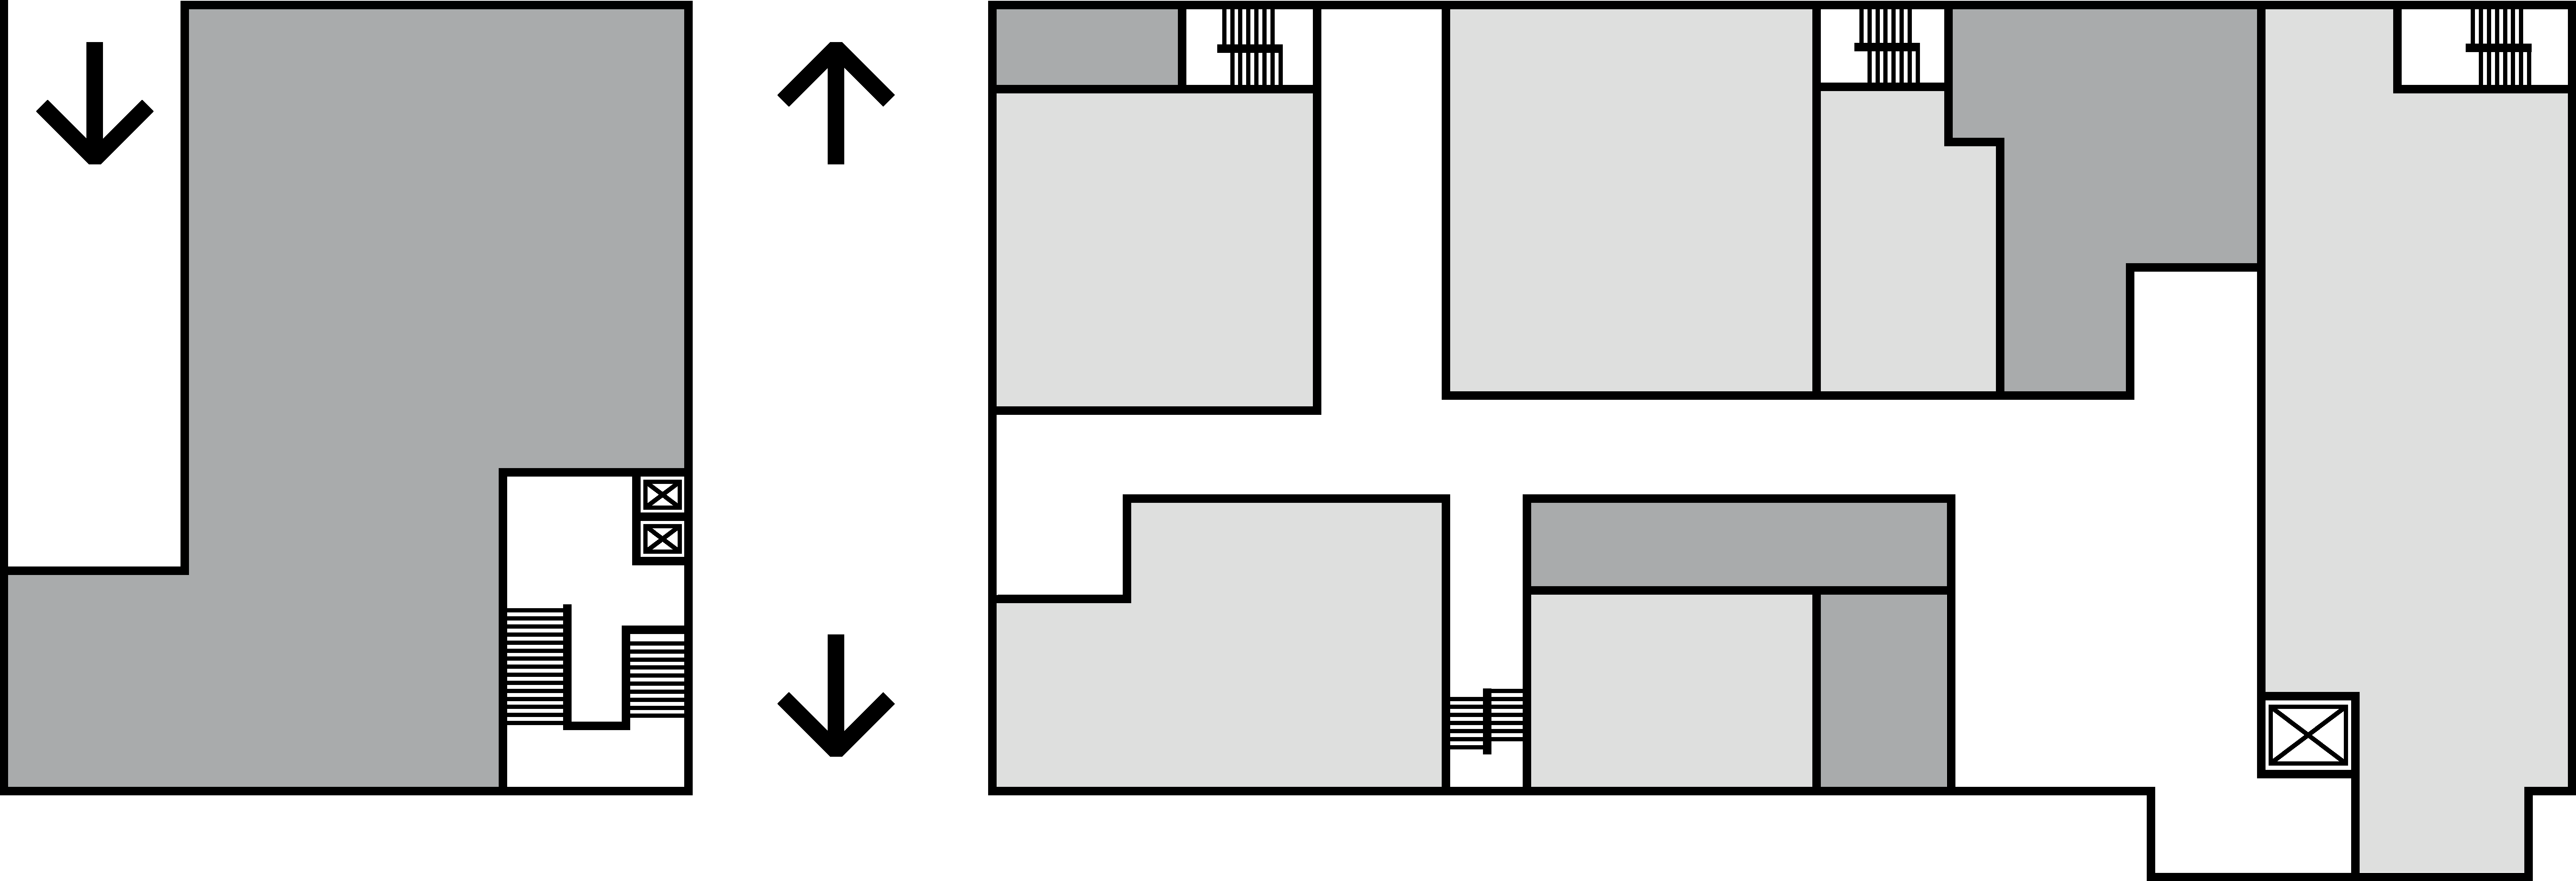
\includegraphics[width=\textwidth]{images/plan.pdf} % angle=90
    };   
    
\node[copyright](cr) at (p2.south west){\footnotesize \textcopyright~ Feki.de};
\node[room] at(33, 84) {00.019};
\node[room] at(48, 82) {00.022};
\node[room] at(60, 83) {\rotatebox{90}{WC}};
\node[room] at(50, 98) {00.043};
\node[room] at(75, 86) {\rotatebox{90}{00.033}};
\node[room] at(78, 84) {\rotatebox{90}{music hall}};
\node[room] at(34, 97) {Cafeteria};
\node[room, font=\scriptsize] at(0, 81) {\rotatebox{90}{underground}};
\node[room, font=\scriptsize] at(3, 84) {\rotatebox{90}{garage}};
\node[room, font=\scriptsize] at(24, 83) {street};
\node[room, font=\scriptsize] at(22, 91) {inner\\ courtyard};

\end{tikzpicture}
\end{center}

\subsection{\textcolor{unibablueI}{Means of Transport}}
\textbf{\textcolor{unibablueII}{Public transport (ÖPNV):}}\\
Bus stop ``Spinnerei'' (line 906, 938)\\
\textbf{\textcolor{unibablueII}{Parking:}}\\
underground garage beneath the university building

\subsection{\textcolor{unibablueI}{Contact}}
An der Weberei 5\\
96047 Bamberg\\[2ex]
Web: www.mmb2014.de